\documentclass{article}
\usepackage[utf8]{inputenc}
\usepackage{amsmath, amssymb, tikz, geometry, multicol}
\usepackage{pgfplots}
\pgfplotsset{compat=1.17}
\geometry{margin=0.5in}
\setlength{\columnsep}{1cm}

\begin{document}

\begin{multicols}{2}

\section*{Lorentz Factor Calculations}

\subsection*{Given}

Set the speed of light:
\[
c = 300
\]

Velocities to consider:
\[
v = 0,\, 1,\, 10,\, 100,\, 300
\]

\subsection*{Calculations}

\begin{enumerate}
    \item Calculate \( v/c \)
    \item Calculate \( \left( \dfrac{v}{c} \right)^2 \)
    \item Calculate \( 1 - \left( \dfrac{v}{c} \right)^2 \)
    \item Calculate \( \sqrt{1 - \left( \dfrac{v}{c} \right)^2} \)
    \item Calculate \( \gamma = \dfrac{1}{\sqrt{1 - \left( \dfrac{v}{c} \right)^2}} \)
\end{enumerate}

\subsection*{Tabulated Results}

\begin{center}
\begin{tabular}{|c|c|c|c|c|c|}
\hline
\( v \) & \( v/c \) & \( \left( \dfrac{v}{c} \right)^2 \) & \( 1 - \left( \dfrac{v}{c} \right)^2 \) & \( \sqrt{1 - \left( \dfrac{v}{c} \right)^2} \) & \( \gamma \) \\
\hline
0 & 0 & 0 & 1 & 1 & 1 \\
\hline
1 & \( \dfrac{1}{300} \approx 0.003333 \) & \( \approx 0.00001111 \) & \( \approx 0.99998889 \) & \( \approx 0.99999444 \) & \( \approx 1.00000556 \) \\
\hline
10 & \( \dfrac{10}{300} \approx 0.033333 \) & \( \approx 0.00111111 \) & \( \approx 0.99888889 \) & \( \approx 0.9994445 \) & \( \approx 1.0005558 \) \\
\hline
100 & \( \dfrac{100}{300} \approx 0.333333 \) & \( \approx 0.11111111 \) & \( \approx 0.88888889 \) & \( \approx 0.942809 \) & \( \approx 1.06066 \) \\
\hline
300 & 1 & 1 & 0 & 0 & Undefined \\
\hline
\end{tabular}
\end{center}

\subsection*{Notes}

- At \( v = c \), the Lorentz factor \( \gamma \) becomes infinite.
- For \( v > c \), the expressions become undefined in real numbers.

\subsection*{Graphs of Each Step}

\subsubsection*{1. Plot of $v$ vs. $v/c$}

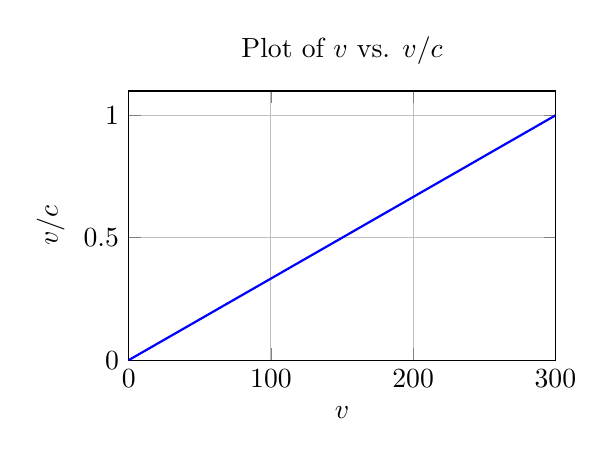
\begin{tikzpicture}
\begin{axis}[
    width=7cm,
    height=5cm,
    xlabel={$v$},
    ylabel={\( v/c \)},
    xmin=0, xmax=300,
    ymin=0, ymax=1.1,
    grid=both,
    title={Plot of $v$ vs. $v/c$}
]
\addplot [domain=0:300, samples=100, thick, blue] {x/300};
\end{axis}
\end{tikzpicture}

\subsubsection*{2. Plot of $v$ vs. $(v/c)^2$}

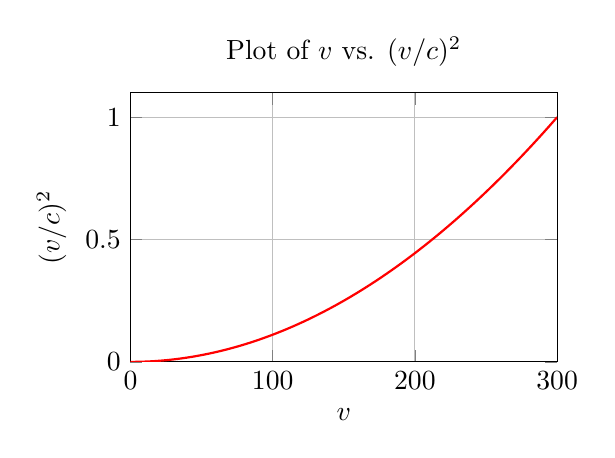
\begin{tikzpicture}
\begin{axis}[
    width=7cm,
    height=5cm,
    xlabel={$v$},
    ylabel={\( (v/c)^2 \)},
    xmin=0, xmax=300,
    ymin=0, ymax=1.1,
    grid=both,
    title={Plot of $v$ vs. $(v/c)^2$}
]
\addplot [domain=0:300, samples=100, thick, red] {(x/300)^2};
\end{axis}
\end{tikzpicture}

\subsubsection*{3. Plot of $v$ vs. $1 - (v/c)^2$}

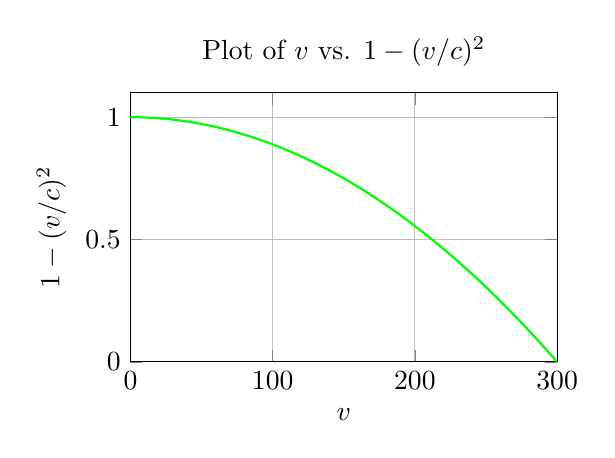
\begin{tikzpicture}
\begin{axis}[
    width=7cm,
    height=5cm,
    xlabel={$v$},
    ylabel={\( 1 - (v/c)^2 \)},
    xmin=0, xmax=300,
    ymin=0, ymax=1.1,
    grid=both,
    title={Plot of $v$ vs. $1 - (v/c)^2$}
]
\addplot [domain=0:300, samples=100, thick, green] {1 - (x/300)^2};
\end{axis}
\end{tikzpicture}

\columnbreak

\subsubsection*{4. Plot of $v$ vs. $\sqrt{1 - (v/c)^2}$}

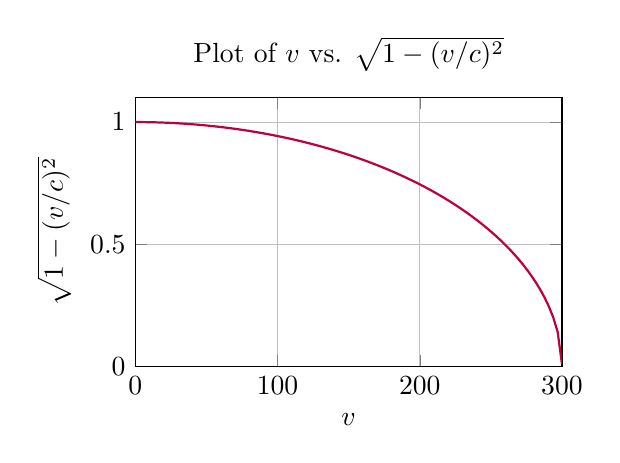
\begin{tikzpicture}
\begin{axis}[
    width=7cm,
    height=5cm,
    xlabel={$v$},
    ylabel={\( \sqrt{1 - (v/c)^2} \)},
    xmin=0, xmax=300,
    ymin=0, ymax=1.1,
    grid=both,
    title={Plot of $v$ vs. $\sqrt{1 - (v/c)^2}$}
]
\addplot [domain=0:300, samples=100, thick, purple] {sqrt(1 - (x/300)^2)};
\end{axis}
\end{tikzpicture}

\subsubsection*{5. Plot of $v$ vs. $\gamma$}

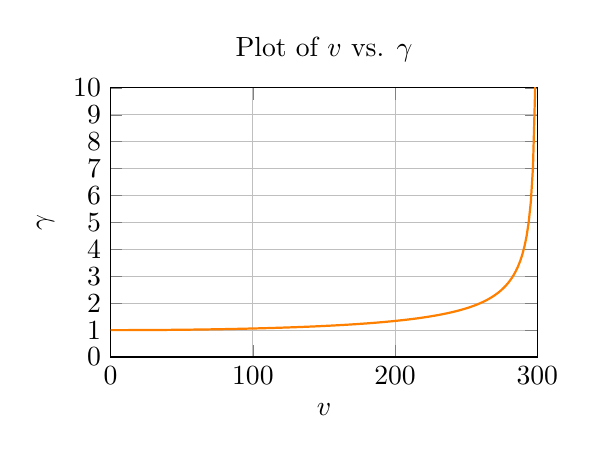
\begin{tikzpicture}
\begin{axis}[
    width=7cm,
    height=5cm,
    xlabel={$v$},
    ylabel={\( \gamma \)},
    xmin=0, xmax=300,
    ymin=0, ymax=10,
    grid=both,
    title={Plot of $v$ vs. $\gamma$},
    ytick={0,1,2,3,4,5,6,7,8,9,10},
]
\addplot [domain=0:299.99, samples=200, thick, orange] {1 / sqrt(1 - (x/300)^2)};
\end{axis}
\end{tikzpicture}

\subsection*{Notes on the Graphs}

- In the plot of \( v \) vs. \( \gamma \), as \( v \) approaches \( c \), \( \gamma \) approaches infinity.
- The graph is plotted up to \( v = 299.99 \) to avoid division by zero at \( v = 300 \).

\subsection*{Interpretation}

- The Lorentz factor \( \gamma \) increases slowly at low velocities and increases rapidly as \( v \) approaches \( c \).
- Time dilation and relativistic effects become significant only when \( v \) is a substantial fraction of \( c \).

\end{multicols}

\end{document}
